\documentclass[9pt]{beamer}

\usepackage{amssymb,amsmath,mathtext}
\usepackage{indentfirst,amsfonts}
\usepackage{makecell,multirow,longtable}
\usepackage{graphicx}
\usepackage{color}
\usepackage{verbatim}


\graphicspath{{graphs/}}

\usepackage[english,russian]{babel}
\usepackage[T2A]{fontenc}
\usepackage[utf8]{inputenc}

\setbeamertemplate{navigation symbols}{}

\usetheme{Boadilla}

\beamersetuncovermixins{\opaqueness<1>{30}}{\opaqueness<2->{25}}

\setbeamerfont{frametitle}{series=\bfseries}
\setbeamerfont{block title}{series=\bfseries}

\begin{document}
\title{Нейросетевой синтез текстур с трендами}
\author{Будакян Я.\,С. \\ Научный руководитель Грачев Е.\,А.}
\date{2017 г.} 

\maketitle

\begin{frame}\frametitle{Введение}
	Задача состоит в построении и обучении искусственной нейронной сети, которая будет способна синтезировать текстуры с трендом.
	В качестве тренда в текстуре подразумевается какое-то заданное изменение статистических свойств изображения, подчиненное некоторой функциональной зависимости. В качестве таких свойств могут выступать, например, интенсивность появления частиц, пористость среды, и т.п.
\end{frame}

\begin{frame}\frametitle{Постановка задачи} 
	Поскольку задача достаточно общая, в работе рассматривается ее сужение:
	\begin{itemize}
		\item В качестве статистического свойства рассматривается интенсивность появления частиц $\lambda$
		\item Тренд направлен вдоль оси x (горизонтальный тренд)
		\item Тренд является линейным: $ \lambda = \lambda_0 + kx $
		\item Обрабатываются монохромные изображения 256 x 256 пикселей
		\item На вход нейросети подается 2 изображения, с интенсивностью частиц слева и справа (при крайних значениях $\lambda$), на выходе ожидается изображение с трендом
	\end{itemize}
\end{frame}

\begin{frame}\frametitle{Пример входных и выходных изображений}
	\begin{figure}
		\begin{minipage}{0.47\linewidth}
			\center{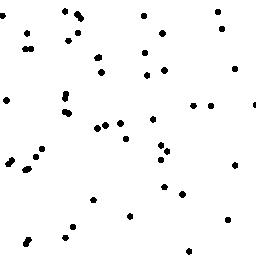
\includegraphics[width=0.6\linewidth]{sampleSide1} \\ Распределение слева \\ (подается на вход)}
		\end{minipage}
		\hfill
		\begin{minipage}{0.47\linewidth}
			\center{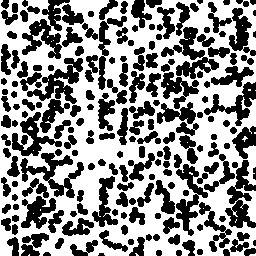
\includegraphics[width=0.6\linewidth]{sampleSide2} \\ Распределение справа \\ (подается на вход)}
		\end{minipage}
		\vfill
		\begin{minipage}{0.47\linewidth}
			\center{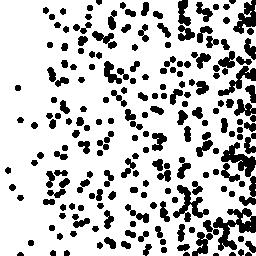
\includegraphics[width=0.6\linewidth]{samplePan} \\ Ожидаемый выход нейросети}
		\end{minipage}
		\hfill
		\begin{minipage}{0.47\linewidth}
			\center{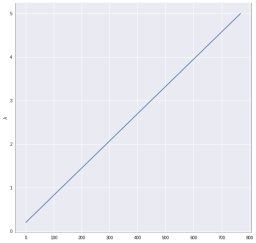
\includegraphics[width=0.6\linewidth]{trend} \\ Тренд интенсивности}
		\end{minipage}
	\end{figure}
\end{frame}

\begin{frame}\frametitle{Математическая постановка задачи}
	Математически задача обучения искусственной нейросети сводится к оптимизации некоторого функционала потерь, конкретный вид которого зависит от выбранной архитектуры сети. На данный момент для решения поставленной задачи я экспериментирую с архитектурой GAN(генеративная состязательная сеть) для которой функционал выглядит следующим образом:
	$$ \mathcal{L}(G, D) = \mathcal{L}_{adv}(G, D) + \eta \mathbb{E}_{s_1, s_2, r \sim p_{data}(s_1, s_2, r)} (\parallel r - G(s_1, s_2) \parallel_1)$$
	$$ \mathcal{L}_{adv}(G, D) = \mathbb{E}_{s_1, s_2, r \sim p_{data}(s_1, s_2, r)}[\log D(s_1, s_2, r)] + $$ $$ + \mathbb{E}_{s_1, s_2 \sim p_{data}(s_1, s_2)} [\log (1 - D(s_1, s_2, G(s_1, s_2)))]$$
	где G, D - ИНС 'генератор' и 'дискриминатор', $(s_1, s_2, r)$ - изображения с интенсивностью слева, справа и реальное изображение с трендом соотвественно,  $\mathbb{E}_{s_1, s_2, r \sim p_{data}(s_1, s_2, r)}$ - математическое ожидание логарифмического правдоподобия того, что тройка изображений $(s_1, s_2, r)$ принадлежит вероятностному распределению реальных троек $p_{data}(s_1, s_2, r)$, а $p_{data}(s_1, s_2)$ соответствует распределению реальных изображений $s_1, s_2$. Оптимизация идет по весам сетей G и D соответственно.
\end{frame}
\end{document}